
The intensive use of generative programming techniques provides an elegant engineering solution to deal with the heterogeneity of platforms and technological stacks. The use of domain-specific languages for example, leads to the creation of numerous code generators that automatically translate high-level system specifications into multi-target executable code. 

Producing correct and efficient code generator is complex and error-prone. Although software designers provide generally high-level test suites to verify the functional outcome of generated code, it remains challenging and tedious to verify the behavior of produced code in terms of non-functional properties.

This chapter describes a black-box testing approach that automatically detect anomalies in code generators in terms of non-functional properties (i.e., resource usage and performance).
 
In fact, we adapt the idea of metamorphic testing to the problem of code generators testing.  Hence, our approach relies on the definition of high level test oracles (i.e., metamorphic relations) to check the potential inefficient code generator among a family of code generators. 

We evaluate our approach by analyzing the performance of Haxe, a popular high-level programming language that involves a set of cross-platform code generators. 
Experimental results show that our approach is able to detect some performance inconsistencies that reveal real issues in Haxe code generators.

This chapter is organized as follows: 

Section 5.1 introduces the context of this work, i.e., the non-functional testing of code generators.

Section 5.2 presents the motivation and background of this work. In particular, we discuss in this section three motivation examples and the problems we are addressing.

Section 5.3 describes the general approach overview and the testing strategy.

In Section 5.4, the evaluation and results of our experiments are discussed. Hence, we provide more details about the experimental settings, the code generators under test, the benchmark used, the evaluation metrics, etc. We discuss then the evaluation results.

Finally, we conclude in Section 5.5. 


\section{Introduction}

Generative programming techniques become a common practice for software development to tame the runtime platform heterogeneity that exists in several domains such as mobile or Internet of Things development. 

The main benefit of using generative programming is to reduce the development and maintenance effort, allowing the development at a higher-level of abstraction through the use of Domain-Specific Languages (DSLs)~\cite{brambilla2012model} for example. 

DSLs, as opposed to general-purpose languages, are high level software languages that focus on specific problem domains. 
DSLs or models are generally coupled with the use of code generators that will automatically transform the manually designed models to software artifacts, which can be deployed on different target platforms. 

However, code generators are known to be very difficult to implement and maintain since they involve a set of complex and heterogeneous technologies~\cite{france2007model,guana2015developers}.

To preserve software reliability and quality, code generators have to respect different requirements. In fact, \textit{non-mature} code generators can generate defective software artifacts which range from uncompilable or semantically dysfunctional code that causes serious damage to the generated software; to non-functional bugs which lead to poor-quality code that can affect system reliability and performance (\eg, high resource usage, high execution time, etc.). 

As a matter of fact, these defects (or also anomalies) should be detected and corrected as early as possible in order to ensure the correct behavior of delivered software.

To check the correctness of the code generation process, developers often define (at design or runtime level) a set of test cases that will verify the functional behavior of generated code. 

After code generation, test suites are executed within each target platform, which may lead to either a correct behavior (\ie, expected output) or incorrect one (\ie, failures, errors).

However, it is possible to generate code where all tests pass but, having a very poor quality design. In this case, the quality of generated code can negatively influence on the non-functional requirements and cause performance issues\cite{hundt2011loop,ray2014large}.

Testing the non-functional properties of code generators is a challenging and time-consuming task because developers need to deploy and run code every time a change is made in order to analyze and verify its non-functional behavior.

This task becomes more tedious when targeting different platforms and software languages. Thus, different platform-specific tools will be needed to track bugs and identify the cause of execution failures~\cite{guana2014chaintracker,delgado2004taxonomy}. 

Currently, there is a lack of automatic solutions that check the non-functional issues such as the properties related to the resource consumption of generated code (Memory or CPU consumption).

%we propose a testing approach based on a runtime monitoring infrastructure to automatically check the potential inefficient code generators. This infrastructure, based on system containers as execution platforms, allows code-generator developers to evaluate the generated code performance. %In fact, we provide a fine-grained understanding of resource consumption and analysis of components behavior. 


In this chapter, we are presenting the following contributions:

\begin{itemize} 	
	
	\item We propose a fully automated black box testing approach for detecting code generator inconsistencies within code generator families. We use metamorphic relations as means of test oracles for our test suites. In this contribution, we focus on detecting anomalies related to performance and resource usage properties.
	
	\item We report the results of an empirical study by evaluating the non-functional properties of the Haxe code generators. 
	Haxe is a popular high-level programming language\footnote{\num{1442} GitHub stars} that involves a set of cross-platform code generators able to generate code to different target platforms. The obtained results provide evidence to support the claim that our proposed approach is able to detect code generator issues.
	

	
\end{itemize}

\section{Motivation}

\subsection{Code Generator Families}
This paper is based on the intuition that a code generator is often a member of a family of code generators.

\begin{mydef}[\textbf{Code generator family}]
	We define a code generator family as a set of code generators that takes as input the same language/model and generate code for different target platforms.
\end{mydef}
%Thus, we can automatically compare the performance between different versions
%of generated code (coming from the same source program). Based on this comparison, we can automatically detect singular resource consumptions that could reveal a code generator bug.
The availability of multiple generators with comparable functionality enables to apply the idea of differential testing~\cite{mckeeman1998differential} to detect code generator issues.
As motivating examples for this research, we can cite three approaches that intensively develop and use code generator families: 
\paragraph{a. Haxe.} 	Haxe\footnote{\url{http://haxe.org/}}~\cite{dasnois2011haxe} is an open source toolkit for cross-platform development which compiles to a number of different programming platforms, including JavaScript, Flash, PHP, C++, C\#, and Java. Haxe involves many features: the Haxe language, multi-platform compilers, and different native libraries. The Haxe language is a high-level programming language which is strictly typed. This language supports both, functional and object-oriented programming paradigms. It has a common type hierarchy, making certain API available on every target platform. Moreover, Haxe comes with a set of code generators that translate manually-written code (in Haxe language) to different target languages and platforms.  
%Haxe code can be compiled for applications running on desktop, mobile, and web platforms. Compilers ensure the correctness of user code in terms of syntax and type safety. Haxe comes also with a set of standard libraries that can be used on all supported targets and platform-specific libraries for each of them. One of the main uses of Haxe is to develop cross-platform games or cross-platform libraries that can run on mobile, on the Web or on a Desktop.  
This project is popular (more than \num{1440} stars on GitHub).

\paragraph{b. ThingML.} ThingML\footnote{\url{http://thingml.org/}} is a modeling language for embedded and distributed systems~\cite{fleurey2011mde}. The idea of ThingML is to develop a practical model-driven software engineering tool-chain which targets resource-constrained embedded systems such as low-power sensors and microcontroller-based devices. ThingML is developed as a domain-specific modeling language which includes concepts to describe both software components and communication protocols. The formalism used is a combination of architecture models, state machines and an imperative action language. The ThingML tool-set provides a  code generator families  to translate ThingML to C, Java and JavaScript. It includes a set of variants for the C and JavaScript code generators to target different embedded systems and their constraints. 
This project is still confidential, but it is a good candidate to represent the modeling community practices.

\paragraph{c. TypeScript.} TypeScript\footnote{\url{https://www.typescriptlang.org/}}is a typed superset of JavaScript that compiles to plain JavaScript~\cite{rastogi2015safe}. In fact, it does not compile to only one version of JavaScript. It can transform TypeScript to EcmaScript 3, 5 or 6. It can generate JavaScript that uses different system modules ('none', 'commonjs', 'amd', 'system', 'umd', 'es6', or 'es2015')\footnote{Each of this variation point can target different code generators (function \textit{emitES6Module} vs \textit{emitUMDModule} in emitter.ts for example).}. 
This project is popular (more than \num{12619} stars on GitHub).


\subsection{Functional Correctness of a Code Generator Family}

A reliable and acceptable way to increase the confidence in the correctness of a code generator family is to validate and check the functionality of generated code, which is a common practice for compiler validation and testing~\cite{jorges2014back,stuermer2007systematic,sturmer2005overview}.
Therefore, developers try to check the syntactic and semantic correctness of the generated code by means of different techniques such as static analysis, test suites, etc., and ensure that the code is behaving correctly.  
Functionally testing a code generator family in this case would be simple. Since the generated programs have the same input program, the oracle can be defined as the comparison between the functional outputs of these programs which should be the same.
%In model-based testing for example~\cite{jorges2014back,stuermer2007systematic}, testing code generators focuses on testing the generated code against its design. Thus, the model and the generated code are executed in parallel, by means of simulations, with the same set of test suites. Afterwards, the two outputs are compared with respect to certain acceptance criteria. Test cases, in this case, can be designed to maximize the code or model coverage~\cite{sturmer2005overview}. 

Based on the three sample projects presented above, we remark that all GitHub code repositories of the corresponding projects use unit tests to check the correctness of code generators.  

\subsection{Performance Evaluation of a Code Generator Family}

Another important aspect of code generators testing is to test the non-functional properties of produced code. 
Code generators have to respect different requirements to preserve software reliability and quality~\cite{demertzi2011analyzing}. 
In this case, ensuring the code quality of generated code can require examining several non-functional properties such as code size, resource or energy consumption, execution time, etc~\cite{pan2006fast}.
A non-efficient code generator might generate defective software artifacts (code smells) that violates common software engineering practices. 
Thus, poor-quality code can affect system reliability and performance (e.g., high resource usage, high execution time, etc.).
Proving that the generated code is functionally correct is not enough to claim the effectiveness of the code generator under test. In looking at the three motivating examples, we can observe that ThingML and TypeScript do not provide any specific tests to check the consistency of code generators regarding the memory or CPU usage properties. Haxe provides two test cases\footnote{https://github.com/HaxeFoundation/haxe/tree/development/tests/benchs} to benchmark the resulting generated code. One serves to benchmark an example in which object allocations are deliberately (over) used to measure how memory access/GC mixes with numeric processing in different target languages. The second test evaluates the network speed across different target platforms.

\subsection{Performance Issues of a Code Generator Family}

The potential issues that can reveal an inefficient code generator can be resumed as following:
\begin{itemize}
	\setlength\itemsep{0em}
	\item  the lack of use of a \textbf{specific function that exists in the standard library} of the target language  that can speed or reduce the memory consumption of the resulting program.
	\item the lack of use of \textbf{a specific type that exists in the standard library} of the target language  that can speed or reduce the memory consumption of the resulting program.
	\item  the lack of use of\textbf{ a specific language feature in a target language}  that can speed or reduce the memory consumption of the resulting program. 
\end{itemize}


The main difficulties with testing the non-functional properties of code generators is that we cannot just observe the execution of produced code, but we have to observe and compare the execution of generated programs with equivalent implementations (i.e., in other languages). Even if there is no explicit oracle to detect inconsistencies, we could benefit from the family of code generators to compare the behavior of several generated programs and detect singular resource consumption profiles that could reveal a code generator bug~\cite{hundt2011loop}. 
Our approach is a black-box testing technique and it does not provide detailed information about the source of the issues, as described above. Nevertheless, we rather provide a mechanism to detect these potential issues within a set of code generator families so that, these issues may be investigated and fixed afterwards by code generators/software maintainers.

Next section discusses the common process used by developers to automatically test the performance of generated code. We also illustrate how we can benefit from the code generators families to identify suspect singular behaviors.


%In short, then, we believe that testing the non-functional properties of code generators remains challenging and time-consuming task because developers have to analyze and verify code for each target platform using platform-dependent tools which makes the task of maintaining code generators very tedious. The heterogeneity of platforms and the diversity of target software languages increase the need of supporting tools that can evaluate the consistency and coherence of generated code regarding the non-functional properties. This paper describes a new approach, based on micro-services as execution platforms, to automate and ease the non-functional testing of code generators. This runtime monitoring infrastructure provides a fine-grained understanding of resource consumption and analysis of generated code's behavior.




%\vspace*{-0.3 cm}

\section{Approach Overview}


\subsection{Non-Functional Testing of a Code Generator Family: a Common Process}

Figure \ref{fig:background.pdf} summarizes the classical steps that ensure the code generation and non-functional testing of produced code from design time to runtime. 
We distinguish 4 major steps: the software design using high-level system specifications, code generation by means of code generators, code execution, and non-functional testing of generated code. 


\begin{figure*}[t]
	\center
	
	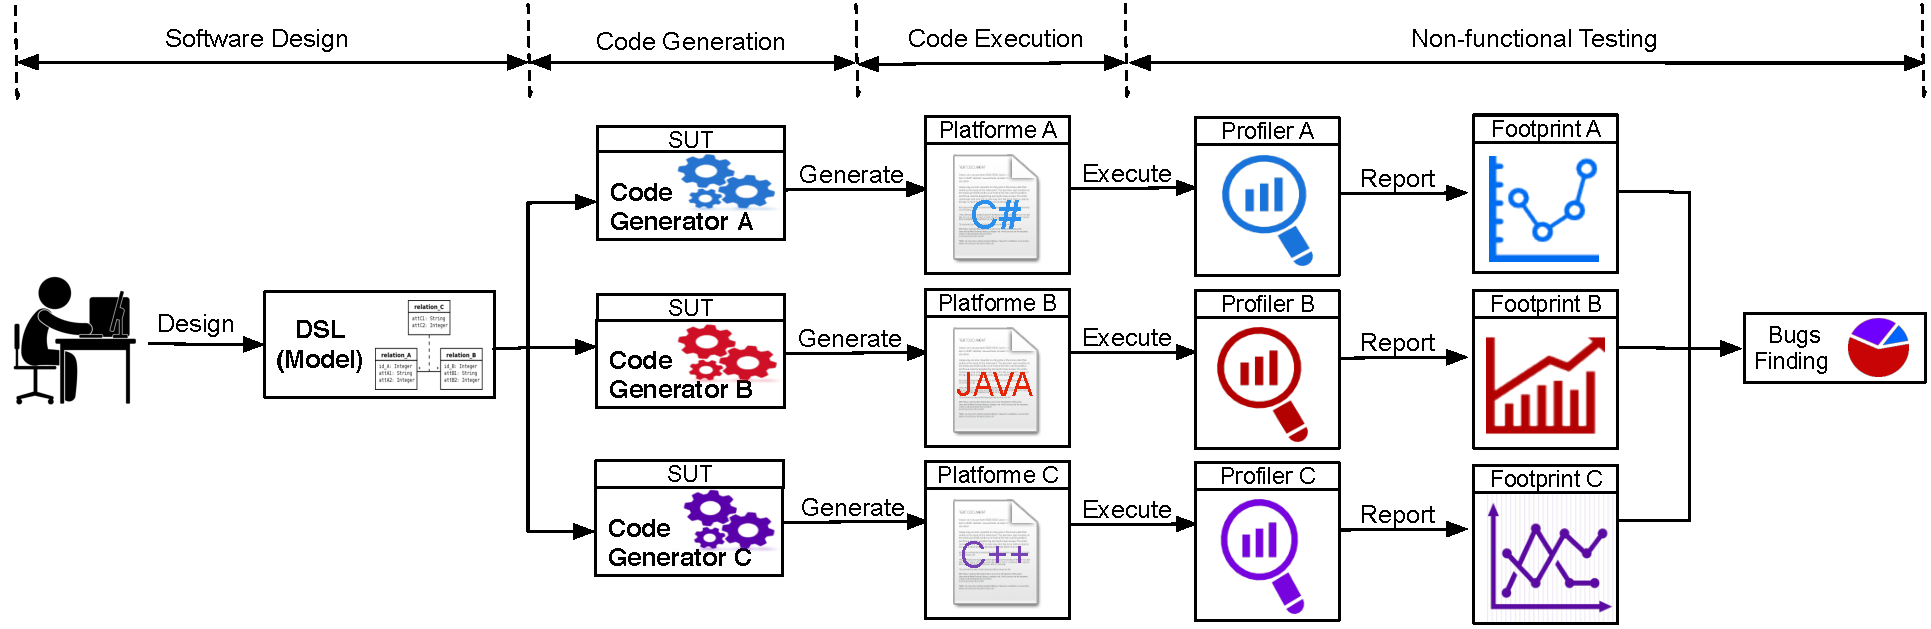
\includegraphics[width=0.95\linewidth]{chapitre4/fig/background.pdf}
	\caption{An overall overview of the different processes involved to ensure the code generation and non-functional testing of produced code from design time to runtime: the classical way}
	\label{fig:background.pdf}
\end{figure*}


In the first step, software developers have to define, at design time, the software's behavior using a high-level abstract language (DSLs, models, program, etc). Afterwards, developers can use platform-specific code generators to ease the software development and automatically generate code for different languages and platforms. We depict, as an example in Figure\ref{fig:background.pdf}, three code generators from the same family capable to generate code to three software programming languages (JAVA, C\# and C++). The first step is to generate code from the previously designed model.
% Transformations from model to code within each code generator might be different and may integrate different transformation rules. As an example, we distinguish model-to-model transformations languages such as ATL~\cite{jouault2005transforming} and template-based model-to-text transformation languages such as Acceleo~\cite{musset2006acceleo} to translate high-level system specifications into executable code and scripts~\cite{bragancca2008transformation,czarnecki2003classification}. The main task of code generators is to transform models to general-purpose and platform-dependent languages.
Afterwards, generated software artifacts (e.g., JAVA, C\#, C++, etc.) are compiled, deployed and executed across different target platforms (e.g., Android, ARM/Linux, JVM, x86/Linux, etc.). 
%Thus, several code compilers are needed to transform source code to machine code (binaries) in order to get executed. 
Finally, to perform the non-functional testing of generated code, developers have to collect, visualize and compare information about the performance and efficiency of running code across the different platforms. 
Therefore, they generally use several platform-specific profilers, trackers, instrumenting and monitoring tools in order to find some inconsistencies or bugs during code execution~\cite{guana2014chaintracker,delgado2004taxonomy}. Finding inconsistencies within code generators involves analyzing and inspecting the code and that, for each execution platform. For example, one way to handle that, is to analyze the memory footprint of software execution and find memory leaks~\cite{nethercote2007valgrind}. Developers can then inspect the generated code and find some fragments of the code-base that have triggered this issue. %Such non-functional error could occur when the code generator produces code that presents for example: incorrect typing, faulty memory management, code-smells, etc. 
Therefore, software testers generally use to report statistics about the performance of generated code in order to fix, refactor, and optimize the code generation process. Compared to this classical testing approach, our proposed work seeks to automate the last three steps: generate code, execute it on top of different platforms, and find code generator issues. 

\subsection{An Infrastructure for Non-functional Testing Using System Containers}
To assess the performance/non-functional properties of generated code many system configurations (i.e., execution environments) must be considered. Running different applications (i.e., generated code) with different configurations on one single machine is complex. 
A single system has limited resources and this can lead to performance regressions. Moreover, each execution environment comes with a collection of appropriate tools such as compilers, code generators, debuggers, profilers, etc. Therefore, we need to deploy the test harness, i.e., the produced binaries, on an elastic infrastructure that provide facilities to the code generator developers to ensure the deployment and monitoring of generated code in different environment settings. 
Consequently, our infrastructure provides support to automatically:
\begin{enumerate}
	\item Deploy the generated code, its dependencies and its  execution environments
	\item Execute the produced binaries in an isolated environment 
	\item Monitor the execution 
	\item Gather performance metrics (CPU, Memory, etc.)
\end{enumerate}

To ensure these four main steps, we rely on system containers~\cite{soltesz2007container}. 
It is an operating system-level virtualization method for running multiple isolated Linux systems (containers) on a control host using a single Linux kernel. 
The Linux kernel provides the cgroups functionality that allows limitation and prioritization of resources (CPU, memory, block I/O, network, etc.) for each container without the need of starting any virtual machines~\cite{luotowards}.
These containers share the same OS and hardware as the hosting machine and it is very useful to use them in order to create new configurable and isolated instances to run. 
With container-based virtualization, we reduce the overhead associated with having each guest running a new installed operating system like using virtual machines. This approach can also improve the performance because there is just one operating system taking care of hardware calls.

%Thus, instead of configuring all code generators under test (GUTs) within the same host machine, we wrap each GUT within a system container. Afterwards, a new instance of the container is created to enable the execution of generated code in an isolated and configured environment. Meanwhile, we start our runtime testing components. A monitoring component collects usage statistics of all running containers and save them at runtime in a time series database component. Thus, we can compare later information about the resource usage of generated programs and detect inconsistencies within code generators.


The rest of this section details the technical choices we have made to synthesize this testing infrastructure.

\subsection{Technical Implementation}

The overall overview of our proposed approach is shown in Figure \ref{fig:background2.pdf}. In the following subsections, we describe the deployment and testing architecture using system containers.


\begin{figure*}[!h]
	\center
	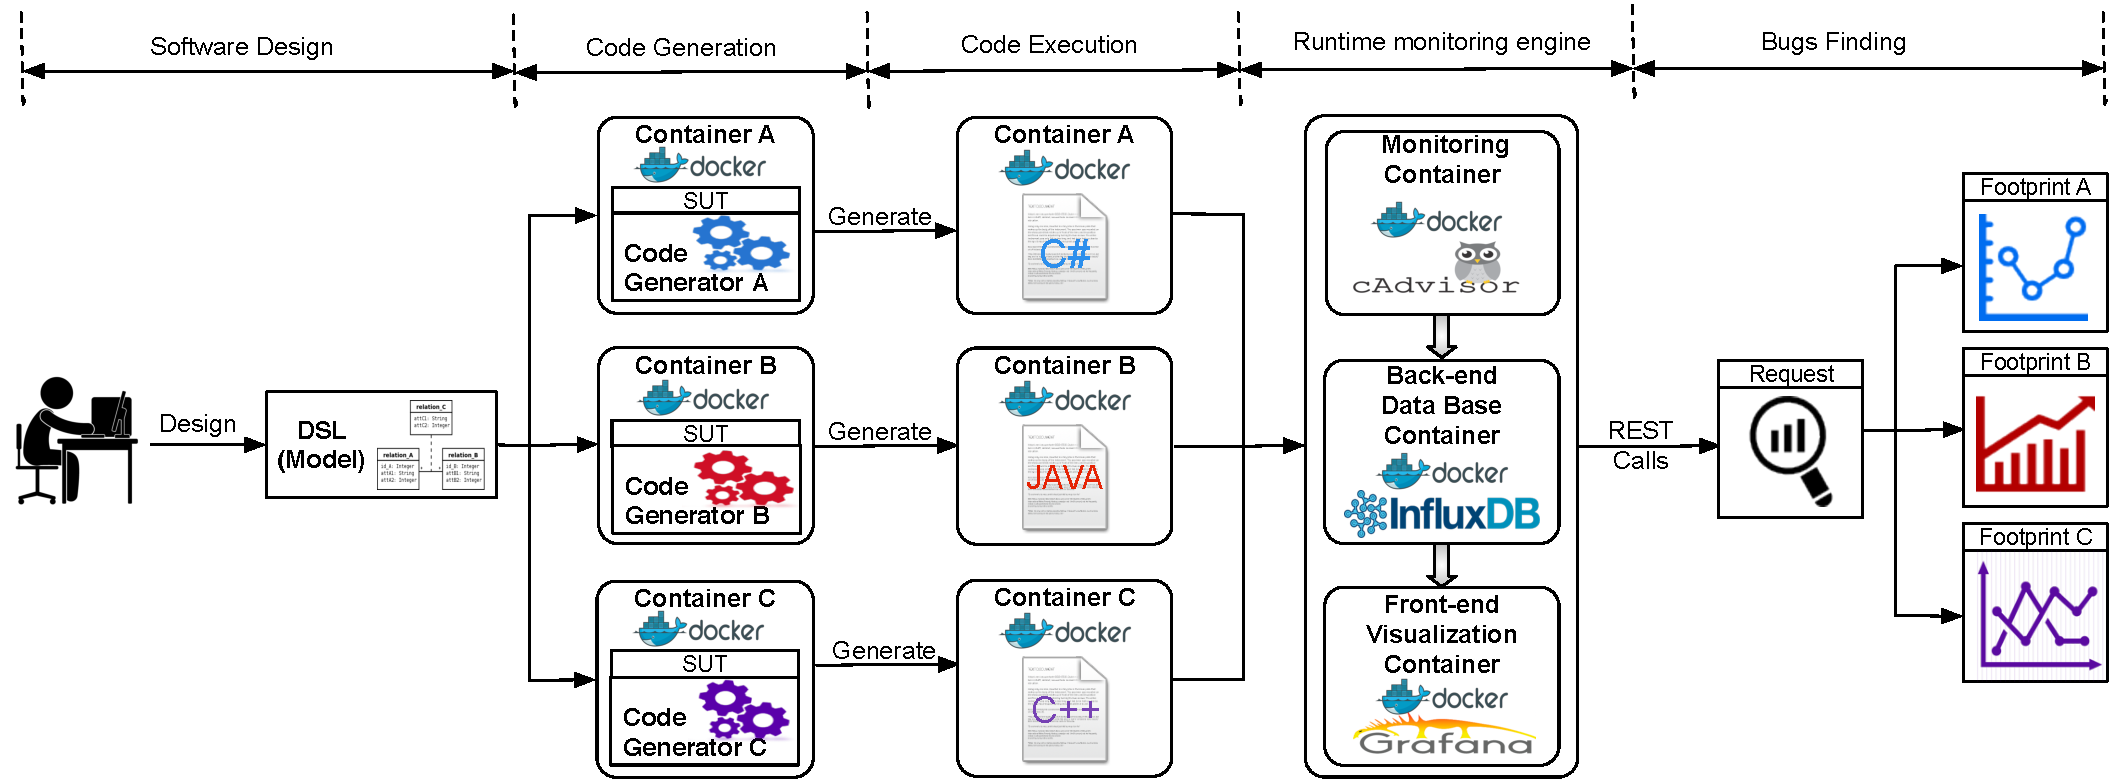
\includegraphics[width=0.95\linewidth]{chapitre4/fig/background2.pdf}
	\caption{A technical overview of the different processes involved to ensure the code generation and non-functional testing of produced code from design time to runtime.}
	\label{fig:background2.pdf}
\end{figure*}


\subsubsection{System Containers as Execution Platforms}


%For this purpose, we propose a testing infrastructure based on System Container techniques such as Docker\footnote{\url{https://www.docker.com}} environment. 
%This framework automates the deployment and execution of applications inside software containers by allowing multiple program configurations to run autonomously on different servers (i. e., a cloud servers).
%It also provides a distributed environment where system storage and resources can be finely managed and limited according to the needs. 

%Thus, we integrate a collection of components to define the adequate infrastructure for testing and monitoring of code generators. 


Before starting to monitor and test applications, we need to deploy the generated code on different components to ease containers provisioning and profiling. 
We aim to use Docker Linux containers to monitor the execution of different generated artifacts in terms of resource usage~\cite{merkel2014docker}. 
Docker\footnote{\url{https://www.docker.com}} is an engine that automates the deployment of any application as a lightweight, portable, and self-sufficient container that runs virtually on a host machine. 
%To achieve that, Docker uses the Linux container technology. 
Using Docker, we can define preconfigured applications and servers to host as virtual images. We can also define the way the service should be deployed in the host machine using configuration files called Docker files. 
In fact, instead of configuring all code generators under test (GUTs) within the same host machine (as shown in Figure~\label{fig:background1.pdf}), our tool wrap each GUT within a container. To do so, we create a new configuration image for each GUT (i.e., the Docker image) where we install all the libraries, compilers, and dependencies needed to ensure the code generation and compilation. Thereby, the GUT produces code within multiple instances of the preconfigured Docker images (see code generation step in Figure~2).
%As properties, we can define the OS where the service has to run, dependencies, etc. 
%A simple way to build images automatically is to use Dockerfiles which represents configuration files.
%Docker can build images automatically by reading the instructions from a Dockerfile. 
We use the public Docker registry\footnote{\url{https://hub.docker.com/}} for  saving, and managing all our Docker images. 
%It represents a cloud-based registry service for building and shipping application or service containers.
We can then instantiate different containers from these Docker images. 
%Basically, each container deploys an optimized version of the input source code program.

Next, each generated code is executed individually inside an isolated Linux container (see code execution step in Figure \ref{fig:background2.pdf}). By doing so, we ensure that each executed program runs in isolation without being affected by the host machine or any other processes. Moreover, since a container is cheap to create, we are able to create new container instances as long as we have new programs to execute.  
Since each program execution requires a new container to be created, it is crucial to remove and kill containers that have finished their job to eliminate the load on the system. We run the experiment on top of a private data-center that provide a bare-metal installation of  docker and docker swarm. On a single machine,  containers/softwares are running sequentially and we pin $p$ cores and $n$ \SI{}{\giga\byte}
of memory for each container\footnote{$p$ and $n$ can be configured}. Once the execution is done, resources reserved for the container are automatically released to enable spawning next containers. Therefore, the host machine will not suffer too much from performance trade-offs.
In short, the main advantages of this approach are:
\begin{itemize}
	\item The use of containers induces less performance overhead compared to using a full stack virtualization solution~\cite{spoiala2016performance}. Indeed, instrumentation and monitoring tools for memory profiling can induce too much overhead.
	\item Thanks to the use of Dockerfiles, the proposed framework can be  configured by software testers in order to define the GUT (\eg, code generator version, dependencies, etc.), the host IP and OS, the DSL design, the optimization options, etc. Thus, we can use the same configured Docker image to execute different instances of generated code. For hardware architecture, containers share the same platform architecture as the host machine (e.g., x86, x64, ARM, etc.). 
	\item Docker uses Linux control groups (Cgroups) to group processes running in the container. This allows us to manage the resources of a group of processes, which is very valuable. 
	This approach increases the flexibility when we want to manage resources since we can manage every group individually. For example, if we would evaluate the non-functional requirements of generated code within a resource-constrained environment, we can  request and limit resources within the execution container according to the needs.
	\item Although containers run in isolation, they can share data with the host machine and other running containers. Thus, non-functional data relative to resource consumption can be gathered and managed by other containers (\ie, for storage purpose, visualization)
\end{itemize}




\subsubsection{Runtime Testing Components}
In order to test our running applications within Docker containers, we aim to use a set of Docker components to ease the extraction of resource usage information (see runtime monitoring engine in Figure~2).
\paragraph{Monitoring Component}
This container provides an understanding of the resource usage and performance characteristics of our running containers. Generally, Docker containers rely on Cgroups file systems to expose a lot of metrics about accumulated CPU cycles, memory, block I/O usage, etc. Therefore, our monitoring component automates the extraction of runtime performance metrics stored in Cgroups files. For example, we access live resource consumption of each container available at the Cgroups file system via stats found in \textit{"/sys/fs/cgroup/cpu/docker/(longid)/"} (for CPU consumption) and \textit{"/sys/fs/cgroup/memory/docker/(longid)/"} (for stats related to memory consumption). This component will automate the process of service discovery and metrics aggregation for each new container. Thus, instead of gathering manually metrics located in Cgroups file systems, it extracts automatically the runtime resource usage statistics relative to the running component (i.e., the generated code that is running within a container). We note that resource usage information is collected in raw data. This process may induce a little overhead because it does  very fine-grained accounting of resource usage on running container. Fortunately, this may not affect the gathered performance values since we run only one version of generated code within each container.
To ease the monitoring process, we integrate cAdvisor, a Container Advisor\footnote{\url{https://github.com/google/cadvisor}}. cAdvisor monitors service containers at runtime. 

However, cAdvisor monitors and aggregates live data over only 60 seconds interval.
%After 60 seconds, new runtime data is updated and automatically displayed within cAdvisor web interface. 
Therefore, we need to record all data over time, from the beginning  of the container's creation, into a time-series database so that, we can run queries and define non-functional metrics from historical data. 
To make gathered data truly valuable for resource usage monitoring, we link our monitoring component to a back-end database component. 



\paragraph{Back-end Database Component}
This component represents a time-series database back-end. It is plugged with the previously described monitoring component to save the non-functional data for long-term retention, analytics and visualization. 
During code execution, resource usage stats are continuously sent to this component. When a container is killed, we are able to access its relative resource usage metrics through the database. We choose a time-series database because we are collecting time-series data that correspond to the resource utilization profiles of programs execution.

We use InfluxDB\footnote{\url{https://github.com/influxdata/influxdb}}, an open source distributed time-series database as a back-end to record data. InfluxDB allows the user to execute SQL-like queries on the database. For example, the following query reports the maximum memory usage of container $"generated\_code\_v1"$ since its creation:

\begin{lstlisting}[
language=SQL,
showspaces=false,
basicstyle=\small,
numberstyle=\small,
commentstyle=\color{gray},
linewidth=\columnwidth
]
select max (memory_usage) from stats 
where container_name='generated_code_v1'
\end{lstlisting}
To give an idea about the data gathered by the monitoring component and stored in the time-series database, we describe in Table \ref{tab:Resource usage metrics recorded in InfluxDB} these collected metrics:
\begin{table}[h]
	\begin{center}
		\resizebox{0.8\columnwidth}{!}{%
			\begin{tabular}{|p{1.4cm}|p{6.6cm}|}
				\hline
				\textbf{Metric} & \textbf{Description} \\
				\hline
				Name & Container Name \\\hline
				
				T & Elapsed time since container's creation \\\hline
				
				Network  &  Stats for network bytes and packets in an out of the container \\\hline
				
				Disk IO &  Disk I/O stats \\\hline
				
				Memory  &  Memory usage \\\hline
				
				CPU &  CPU usage \\
				\hline
				
			\end{tabular}%
		}
		
	\end{center}
	\caption {Resource usage metrics recorded in InfluxDB}
	\label{tab:Resource usage metrics recorded in InfluxDB}
	%\vspace*{-0.9cm}
\end{table}

Apart from that, our framework provides also information about the size of generated binaries and the compilation time needed to produce code.
For instance, resource usage statistics are collected and stored using these two components. It is relevant to show resource usage profiles of running programs overtime. To do so, we present a front-end visualization component for performance profiling. 

\paragraph{Front-end Visualization Component}
%Once we gather and store resource usage data, the next step is visualizing them. That is the role of the visualization component. It will be the endpoint component that we use to visualize the recorded data. 
Once we gather and store resource usage data, the next step is visualizing them. That is the role of the visualization component. It will be the endpoint component that we use to visualize the recorded data. Therefore, we provide a dashboard to run queries and view different profiles of resource consumption of running components through web UI. Thereby, we can compare visually the profiles of resource consumption among containers. Moreover, we use this component to export the data currently being viewed into static CSV document. So, we can perform statistical analysis on this data to detect inconsistencies or performance anomalies (see bugs finding step in Figure~2).
%Moreover, we use this component to export the data currently being viewed into static CSV document. 
%Thereby, we can perform statistical analysis and process data to analyze performance behavior. 
%An overview of the monitoring dashboard is shown in Figure 3.
As a visualization component, we use Grafana\footnote{\url{https://github.com/grafana/grafana}}, a time-series visualization tool available for Docker. 




%\begin{remark}
%	We would notice that this testing infrastructure can be generalized and adapted to other case studies other than code generators. Using system containers, any software application/generated code can be easily deployed within containers (i.e., by configuring the container image). It will be later executed and monitored using our runtime monitoring engine. 
%\end{remark}



\section{Evaluation}
So far, we have presented an automated component-based framework for extracting the performance properties of generated code. In this section, we evaluate the implementation of our approach by explaining the design of our empirical study and the different methods we used to assess the effectiveness of our approach. 
The experimental material is available for replication purposes\footnote{\url{https://testingcodegenerators.wordpress.com/}}.
\subsection{Experimental Setup}
\subsubsection{Code Generators Under Test: Haxe Compilers}
In order to test the applicability of our approach, we conduct experiments on a popular high-level programming language called Haxe and its code generators. 
%Haxe is an open source toolkit for cross-platform development which compiles to a number of different programming platforms, including JavaScript, Flash, PHP, C++, C\# and Java. Haxe involves many features: the Haxe language, multi-platform compilers, and different native libraries. 
%The Haxe language is a high-level programming language which is strictly typed. This language supports both functional programming and object-oriented programming paradigms. It has a common type hierarchy, making certain API available on every targeted platform.
Haxe comes with a set of compilers that translate manually-written code (in Haxe language) to different target languages and platforms. 
%Haxe code can be compiled for applications running on desktop, mobile and web platforms. Compilers ensure the correctness of user code in terms of syntax and type safety.
%Haxe comes also with a set of standard libraries that can be used on all supported targets and platform-specific libraries for each of them.

The process of code transformation and generation can be described as following: Haxe compilers analyze the source code written in Haxe language. Then, the code is checked and parsed into a typed structure, resulting in a typed abstract syntax tree (AST). This AST is optimized and transformed afterwards to produce source code for the target platform/language.
Haxe offers the option of choosing which platform to target for each program using command-line options. Moreover, some optimizations and debugging information can be enabled through command-line interface, but in our experiments, we did not turn on any further options. 

\subsubsection{Cross-platform Benchmark}
One way to prove the effectiveness of our approach is to create benchmarks. Thus, we use the Haxe language and its code generators to build a cross-platform benchmark. The proposed benchmark is composed of a collection of cross-platform libraries that can be compiled to different targets. In these experiments, we consider five Haxe GUTs: Java, JS, C++, CS, and PHP code generators. To select cross-platform libraries, we explore github and we use the Haxe library repository\footnote{\url{http://thx-lib.org/}}. So, we select seven libraries that provide a set of test suites with high code coverage scores. 

In fact, each Haxe library comes with an API and a set of test suites. These tests, written in Haxe, represent a set of unit tests that covers the different functions of the API. The main task of these tests is to check the correct functional behavior of generated programs. To prepare our benchmark, we remove all the tests that fail to compile to our five targets (i.e., errors, crashes and failures) and we keep only test suites that are functionally correct in order to focus only on the non-functional properties.
Moreover, we add manually new test cases to some libraries in order to extend the number of test suites. The number of test suites depends on the number of existing functions within the Haxe library.
We use then these test suites to transform functional tests into stress tests. This can be useful to study the impact of this load on the non-functional properties of generated code such as the performance and resource usage. For example, if one test suite consumes a lot of resources for a specific target, then this could be explained by the fact that the GUT has produced code that is very greedy in terms of resources.
Thus, we run each test suite 1K times to get comparable values in terms of resource usage.
Table \ref{tab:Description of selected benchmark libraries} describes the Haxe libraries that we have selected in this benchmark to evaluate our
approach.

\begin{table}[h]
	\centering
	\resizebox{0.8\columnwidth}{!}{%
		\begin{tabular}{|c|c|p{4.3cm}|}
			
			\hline
			\textbf{Library} & \textbf{\#TestSuites} & \textbf{Description} \\
			\hline
			Color  &  19 &  Color conversion from/to any color space   \\ \hline
			Core & 51  & Provides extensions to many types  \\ \hline
			Hxmath & 6  & A 2D/3D math library  \\ \hline
			Format  &  4 & Format library such as dates, number formats   \\ \hline
			Promise & 3  & Library for lightweight promises and futures  \\ \hline
			Culture & 4  & Localization library for Haxe \\ \hline
			Math & 3  & Generation of random values \\ \hline
		\end{tabular}
	}
	\caption{Description of selected benchmark libraries}
	\label{tab:Description of selected benchmark libraries}
\end{table}

\subsubsection{Evaluation Metrics Used}
We use to evaluate the efficiency of generated code using the following non-functional metrics:

-\textit{Memory usage}:
It corresponds to the maximum memory consumption of the running container under test. Memory usage is measured in \SI{}{\mega\byte}

-\textit{Execution time}:
Program execution time is measured in seconds.

We recall that our tool is able to evaluate other non-functional properties of generated code such as code generation time, compilation time, code size, CPU usage. We choose to focus, in this experiment, on the performance (i.e., execution time) and resource usage (i.e., memory usage).

\subsubsection{Setting up Infrastructure}
\begin{figure}[h]
	\centering
	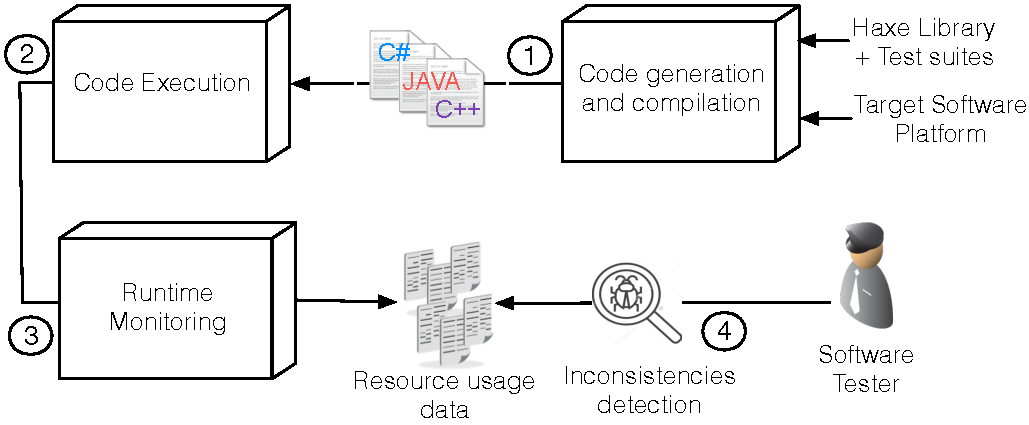
\includegraphics[width=1\linewidth]{chapitre4/fig/settingup.pdf}
	\caption{Infrastructure settings for running experiments}
	\label{fig:settingup.pdf}
\end{figure}
To assess our approach, we configure our previously proposed container-based infrastructure in order to run experiments on the Haxe case study.
Figure \ref{fig:settingup.pdf} shows a big picture of the testing and monitoring infrastructure considered in these experiments.


\begin{table}[h]
	\centering
	
	\resizebox{\columnwidth}{!}{%
		\begin{tabular}{|l|l|S[table-format=3.2]|l|S[table-format=3.2]|l|S[table-format=3.2]|}
			\hline
			\textbf{Benchmark}                 & \textbf{TestSuite} & \textbf{Std\_dev}                & \textbf{TestSuite} & \textbf{Std\_dev}             & \textbf{TestSuite} & \textbf{Std\_dev}              \\ \hline
			& \textbf{TS1}       & 0.55                             & \textbf{TS8}       & 0.24                          & \textbf{TS15}      & 0.73                           \\ \cline{2-7} 
			& \textbf{TS2}       & 0.29                             & \textbf{TS9}       & 0.22                          & \textbf{TS16}      & 0.12                           \\ \cline{2-7} 
			& \textbf{TS3}       & 0.34                             & \textbf{TS10}      & 0.10                          & \textbf{TS17}      & 0.31                           \\ \cline{2-7} 
			& \textbf{TS4}       & 2.51                             & \textbf{TS11}      & 0.17                          & \textbf{TS18}      & 0.34                           \\ \cline{2-7} 
			& \textbf{TS5}       & 1.53                             & \textbf{TS12}      & 0.28                          & \textbf{TS19}      & \cellcolor[HTML]{C0C0C0}120.61 \\ \cline{2-7} 
			& \textbf{TS6}       & 43.50                            & \textbf{TS13}      & 0.33                         & \multicolumn{2}{l|}{\multirow{2}{*}{}} \\ \cline{2-5}
			\multirow{-7}{*}{\textbf{Color}}   & \textbf{TS7}       & 0.50                             & \textbf{TS14}      & 1.88                          & \multicolumn{2}{l|}{}                  \\ \hline
			& \textbf{TS1}       & 0.35                             & \textbf{TS18}      & 0.16                          & \textbf{TS35}      & 1.30                           \\ \cline{2-7} 
			& \textbf{TS2}       & 0.07                             & \textbf{TS19}      & 0.60                          & \textbf{TS36}      & 1.13                           \\ \cline{2-7} 
			& \textbf{TS3}       & 0.30                             & \textbf{TS20}      & 5.79                          & \textbf{TS37}      & 2.02                           \\ \cline{2-7} 
			& \textbf{TS4}       & \cellcolor[HTML]{C0C0C0}27299.89 & \textbf{TS21}      & 0.47                          & \textbf{TS38}      & 0.26                           \\ \cline{2-7} 
			& \textbf{TS5}       & 6.12                             & \textbf{TS22}      & 2.74                          & \textbf{TS39}      & 0.16                           \\ \cline{2-7} 
			& \textbf{TS6}       & 21.90                            & \textbf{TS23}      & 2.14                          & \textbf{TS40}      & 8.12                           \\ \cline{2-7} 
			& \textbf{TS7}       & 0.41                             & \textbf{TS24}      & 3.79                          & \textbf{TS41}      & 5.45                           \\ \cline{2-7} 
			& \textbf{TS8}       & 0.28                             & \textbf{TS25}      & 0.19                          & \textbf{TS42}      & 0.11                           \\ \cline{2-7} 
			& \textbf{TS9}       & 0.78                             & \textbf{TS26}      & 0.13                          & \textbf{TS43}      & 1.41                           \\ \cline{2-7} 
			& \textbf{TS10}      & 1.82                             & \textbf{TS27}      & 5.59                          & \textbf{TS44}      & 1.56                           \\ \cline{2-7} 
			& \textbf{TS11}      & \cellcolor[HTML]{C0C0C0}180.68   & \textbf{TS28}      & 1.71                          & \textbf{TS45}      & 0.11                           \\ \cline{2-7} 
			& \textbf{TS12}      & \cellcolor[HTML]{C0C0C0}185.02   & \textbf{TS29}      & 0.26                          & \textbf{TS46}      & 1.04                           \\ \cline{2-7} 
			& \textbf{TS13}      & \cellcolor[HTML]{C0C0C0}128.78   & \textbf{TS30}      & 0.44                          & \textbf{TS47}      & 0.23                           \\ \cline{2-7} 
			& \textbf{TS14}      & 0.71                             & \textbf{TS31}      & 1.71                          & \textbf{TS48}      & 1.34                           \\ \cline{2-7} 
			& \textbf{TS15}      & 0.12                             & \textbf{TS32}      & 2.42                          & \textbf{TS49}      & 1.86                           \\ \cline{2-7} 
			& \textbf{TS16}      & 0.65                             & \textbf{TS33}      & 8.29                          & \textbf{TS50}      & 1.28                           \\ \cline{2-7} 
			\multirow{-17}{*}{\textbf{Core}}   & \textbf{TS17}      & 0.26                             & \textbf{TS34}      & 5.25                          & \textbf{TS51}      & 3.53                           \\ \hline
			& \textbf{TS1}       & 31.65                            & \textbf{TS3}       & 30.34                         & \textbf{TS5}       & 0.40                           \\ \cline{2-7} 
			\multirow{-2}{*}{\textbf{Hxmath}}  & \textbf{TS2}       & 4.27                             & \textbf{TS4}       & 0.25                          & \textbf{TS6}       & 0.87                           \\ \hline
			& \textbf{TS1}       & 0.28                             & \textbf{TS3}       & \cellcolor[HTML]{C0C0C0}95.36 & \textbf{TS4}       & 1.49                           \\ \cline{2-7} 
			\multirow{-2}{*}{\textbf{Format}}  & \textbf{TS2}       & \cellcolor[HTML]{C0C0C0}64.94    & \multicolumn{4}{l|}{\textbf{}}                                                                           \\ \hline
			\textbf{Promise}                   & \textbf{TS1}       & 0.29                             & \textbf{TS2}       & 13.21                         & \textbf{TS3}       & 1.21                           \\ \hline
			& \textbf{TS1}       & 0.13                             & \textbf{TS3}       & 0.13                          & \textbf{TS4}       & 1.40                           \\ \cline{2-7} 
			\multirow{-2}{*}{\textbf{Culture}} & \textbf{TS2}       & 0.10                             & \multicolumn{4}{l|}{}                                                                                    \\ \hline
			\textbf{Math}                      & \textbf{TS1}       & \cellcolor[HTML]{C0C0C0}642.85   & \textbf{TS2}       & 28.32                         & \textbf{TS3}       & 24.40                          \\ \hline
		\end{tabular}%
	}
	
	\caption{The comparison results of running each test suite across five target languages: the metric used is the standard deviation between execution times  }
	\label{tab:The comparison results1}
\end{table}

% Please add the following required packages to your document preamble:
% \usepackage{multirow}
% Please add the following required packages to your document preamble:
% \usepackage{multirow}
% \usepackage[table,xcdraw]{xcolor}
% If you use beamer only pass "xcolor=table" option, i.e. \documentclass[xcolor=table]{beamer}
\begin{table}[]
	\centering
	
	\resizebox{\columnwidth}{!}{%
		\begin{tabular}{|l|l|S[table-format=3.2]|l|S[table-format=3.2]|l|S[table-format=3.2]|}
			\hline
			\textbf{Benchmark}                 & \textbf{TestSuite} & \textbf{Std\_dev}               & \textbf{TestSuite} & \textbf{Std\_dev}              & \textbf{TestSuite} & \textbf{Std\_dev}              \\ \hline
			& \textbf{TS1}       & 10.19                           & \textbf{TS8}       & 1.23                           & \textbf{TS15}      & 14.44                          \\ \cline{2-7} 
			& \textbf{TS2}       & 1.17                            & \textbf{TS9}       & 1.95                           & \textbf{TS16}      & 1.13                           \\ \cline{2-7} 
			& \textbf{TS3}       & 0.89                            & \textbf{TS10}      & 1.27                           & \textbf{TS17}      & 0.72                           \\ \cline{2-7} 
			& \textbf{TS4}       & 30.34                           & \textbf{TS11}      & 0.57                           & \textbf{TS18}      & 0.97                           \\ \cline{2-7} 
			& \textbf{TS5}       & 31.79                           & \textbf{TS12}      & 1.11                           & \textbf{TS19}      & \cellcolor[HTML]{C0C0C0}777.32 \\ \cline{2-7} 
			& \textbf{TS6}       & \cellcolor[HTML]{C0C0C0}593.05  & \textbf{TS13}      & 0.46                           & \multicolumn{2}{l|}{}                               \\ \cline{2-5}
			\multirow{-7}{*}{\textbf{Color}}   & \textbf{TS7}       & 12.14                           & \textbf{TS14}      & 45.90                          & \multicolumn{2}{l|}{\multirow{-2}{*}{}}             \\ \hline
			& \textbf{TS1}       & 1.40                            & \textbf{TS18}      & 1.00                           & \textbf{TS35}      & 14.13                          \\ \cline{2-7} 
			& \textbf{TS2}       & 1.17                            & \textbf{TS19}      & 20.37                          & \textbf{TS36}      & 32.41                          \\ \cline{2-7} 
			& \textbf{TS3}       & 0.60                            & \textbf{TS20}      & 128.23                         & \textbf{TS37}      & 22.72                          \\ \cline{2-7} 
			& \textbf{TS4}       & \cellcolor[HTML]{C0C0C0}403.15  & \textbf{TS21}      & 24.38                          & \textbf{TS38}      & 2.19                           \\ \cline{2-7} 
			& \textbf{TS5}       & 41.95                           & \textbf{TS22}      & 76.24                          & \textbf{TS39}      & 0.26                           \\ \cline{2-7} 
			& \textbf{TS6}       & 203.55                          & \textbf{TS23}      & 18.82                          & \textbf{TS40}      & 126.29                         \\ \cline{2-7} 
			& \textbf{TS7}       & 19.69                           & \textbf{TS24}      & 72.01                          & \textbf{TS41}      & 31.01                          \\ \cline{2-7} 
			& \textbf{TS8}       & 0.78                            & \textbf{TS25}      & 0.21                           & \textbf{TS42}      & 0.93                           \\ \cline{2-7} 
			& \textbf{TS9}       & 30.41                           & \textbf{TS26}      & 2.30                           & \textbf{TS43}      & 50.36                          \\ \cline{2-7} 
			& \textbf{TS10}      & 57.19                           & \textbf{TS27}      & 101.53                         & \textbf{TS44}      & 12.56                          \\ \cline{2-7} 
			& \textbf{TS11}      & 68.92                           & \textbf{TS28}      & 43.67                          & \textbf{TS45}      & 0.91                           \\ \cline{2-7} 
			& \textbf{TS12}      & 74.19                           & TS29               & 0.90                           & \textbf{TS46}      & 27.28                          \\ \cline{2-7} 
			& \textbf{TS13}      & 263.99                          & \textbf{TS30}      & 4.02                           & \textbf{TS47}      & 1.10                           \\ \cline{2-7} 
			& \textbf{TS14}      & 19.89                           & \textbf{TS31}      & 52.35                          & \textbf{TS48}      & 15.40                          \\ \cline{2-7} 
			& \textbf{TS15}      & 0.30                            & \textbf{TS32}      & 134.75                         & \textbf{TS49}      & 37.01                          \\ \cline{2-7} 
			& \textbf{TS16}      & 28.29                           & \textbf{TS33}      & 82.66                          & \textbf{TS50}      & 23.29                          \\ \cline{2-7} 
			\multirow{-17}{*}{\textbf{Core}}            & \textbf{TS17}      & 1.16                            & \textbf{TS34}      & 89.57                          & \textbf{TS51}      & 1.28                           \\ \hline
			& \textbf{TS1}       & \cellcolor[HTML]{C0C0C0}444.18  & \textbf{TS3}       & \cellcolor[HTML]{C0C0C0}425.65 & \textbf{TS5}       & 17.69                          \\ \cline{2-7} 
			\multirow{-2}{*}{\textbf{Hxmath}}  & \textbf{TS2}       & 154.80                          & \textbf{TS4}       & 0.96                           & \textbf{TS6}       & 46.13                          \\ \hline
			& \textbf{TS1}       & 0.74                            & \textbf{TS3}       & 255.36                         & \textbf{TS4}       & 8.40                           \\ \cline{2-7} 
			\multirow{-2}{*}{\textbf{Format}}  & \textbf{TS2}       & 106.87                          & \multicolumn{4}{l|}{\textbf{}}                                                                            \\ \hline
			\textbf{Promise}                   & \textbf{TS1}       & 0.30                            & \textbf{TS2}       & 58.76                          & \textbf{TS3}       & 20.04                          \\ \hline
			& \textbf{TS1}       & 1.28                            & \textbf{TS3}       & 0.58                           & \textbf{TS4}       & 15.69                          \\ \cline{2-7} 
			\multirow{-2}{*}{\textbf{Culture}} & \textbf{TS2}       & 4.51                            & \multicolumn{4}{l|}{}                                                                                     \\ \hline
			\textbf{Math}                      & \textbf{TS1}       & \cellcolor[HTML]{C0C0C0}1041.53 & \textbf{TS2}       & 234.93                         & \textbf{TS3}       & 281.12                         \\ \hline
		\end{tabular}%
	}
	
	\caption{The comparison results of running each test suite across five target languages: the metric used is the standard deviation between memory consumptions}
    \label{tab:The comparison results2}
\end{table}



\begin{table*}[h]
	\centering
	
	\resizebox{0.75\linewidth}{!}{%
		\begin{tabular}{|l|S[table-format=3.2]|S[table-format=3.2]|S[table-format=3.2]|S[table-format=3.2]|S[table-format=3.2]|S[table-format=3.2]|S[table-format=3.2]|S[table-format=3.2]|S[table-format=5.2]|S[table-format=3.2]|}
			\hline
			\multirow{2}{*}{}    & \multicolumn{2}{c|}{\textbf{JS}}   & \multicolumn{2}{c|}{\textbf{JAVA}} & \multicolumn{2}{c|}{\textbf{C++}}  & \multicolumn{2}{c|}{\textbf{CS}}   & \multicolumn{2}{c|}{\textbf{PHP}}  \\ \cline{2-11} 
			& \textbf{Time(s)} & \textbf{Factor} & \textbf{Time(s)} & \textbf{Factor} & \textbf{Time(s)} & \textbf{Factor} & \textbf{Time(s)} & \textbf{Factor} & \textbf{Time(s)} & \textbf{Factor} \\ \hline
			\textbf{Color\_TS19} & 4.52             & x1.0            & 8.61             & x1.9            & 10.73            & x2.4            & 14.99            & x3.3            & 279.27           & x61.8           \\ \hline
			\textbf{Core\_TS4}   & 665.78           & x1.0            & 416.85           & x0.6            & 699.11           & x1.1            & 1161.29          & x1.7            & 61777.21         & x92.8           \\ \hline
			\textbf{Core\_TS11}  & 4.27             & x1.0            & 1.80             & x0.4            & 1.57             & x0.4            & 5.71             & x1.3            & 407.33           & x95.4           \\ \hline
			\textbf{Core\_TS12}  & 4.71             & x1.0            & 2.06             & x0.4            & 1.60             & x0.3            & 5.36             & x1.1            & 417.14           & x88.6           \\ \hline
			\textbf{Core\_TS13}  & 6.26             & x1.0            & 5.91             & x0.9            & 11.04            & x1.8            & 14.14            & x2.3            & 297.21           & x47.5           \\ \hline
			\textbf{Format\_TS2}   & 2.31             & x1.0            & 2.10             & x0.9            & 1.81             & x0.8            & 6.08             & x2.6            & 148.24           & x64.1           \\ \hline
			\textbf{Format\_TS3}   & 5.40             & x1.0            & 5.03             & x0.9            & 7.67             & x1.4            & 12.38            & x2.3            & 220.76           & x40.9           \\ \hline
			\textbf{Math\_TS1}   & 3.01             & x1.0            & 12.51            & x4.2            & 16.30            & x5.4            & 14.14            & x4.7            & 1448.90          & x481.7          \\ \hline
		\end{tabular}%
	}
	\caption{Raw data values of test suites that led to the highest variation in terms of execution time}
	\label{tab:raw results1}
\end{table*}


\begin{table*}[h]
	\centering
	
	\resizebox{0.75\linewidth}{!}{%
		\begin{tabular}{|l|S[table-format=3.2]|S[table-format=3.2]|S[table-format=3.2]|S[table-format=3.2]|S[table-format=3.2]|S[table-format=3.2]|S[table-format=3.2]|S[table-format=3.2]|S[table-format=3.2]|S[table-format=3.2]|}
			\hline
			\multirow{2}{*}{}    & \multicolumn{2}{c|}{\textbf{JS}}      & \multicolumn{2}{c|}{\textbf{JAVA}}    & \multicolumn{2}{c|}{\textbf{C++}}     & \multicolumn{2}{c|}{\textbf{CS}}      & \multicolumn{2}{c|}{\textbf{PHP}}     \\ \cline{2-11} 
			& \textbf{Memory(Mb)} & \textbf{Factor} & \textbf{Memory(Mb)} & \textbf{Factor} & \textbf{Memory(Mb)} & \textbf{Factor} & \textbf{Memory(Mb)} & \textbf{Factor} & \textbf{Memory(Mb)} & \textbf{Factor} \\ \hline
			\textbf{Color\_TS6}  & 900.70              & x1.0            & 1362.55              & x1.5            & 2275.49             & x2.5            & 1283.31             & x1.4            & 758.79              & x0.8            \\ \hline
			\textbf{Color\_TS19} & 253.01              & x1.0            & 819.92              & x3.2            & 923.99              & x3.7            & 327.61              & x1.3            & 2189.86             & x8.7            \\ \hline
			\textbf{Core\_TS4}   & 303.09              & x1.0            & 768.22              & x2.5            & 618.42              & x2              & 235.75              & x0.8            & 1237.15             & x4.1            \\ \hline
			\textbf{Hxmath\_TS1} & 104.00              & x1.0            & 335.50              & x3.2            & 296.43              & x2.9            & 156.41              & x1.5            & 1192.98             & x11.5           \\ \hline
			\textbf{Hxmath\_TS3} & 111.68              & x1.0            & 389.73              & x3.5            & 273.12              & x2.4            & 136.49              & x1.2            & 1146.05             & x10.3           \\ \hline
			\textbf{Math\_TS1}   & 493.66              & x1.0            & 831.44              & x1.7            & 1492.97             & x3              & 806.33              & x1.6            & 3088.15             & x6.3            \\ \hline
		\end{tabular}%
	}
	\caption{Raw data values of test suites that led to the highest variation in terms of memory usage}
	\label{tab:raw results2}
\end{table*}



First, we create a new Docker image in where we install the Haxe code generators and compilers (through the configuration file "Dockerfile"). Then a new instance of that image is created. It takes as an input the Haxe library we would to test and the list of test suites (step 1). It produces as an output the source code for specific software platforms. These files are saved in a shared repository.
In Docker environment, this repository is called "data volume". A data volume is a specially-designated directory within containers that shares data with the host machine. 
%So, when we execute the generated test suites, we provide a shared volume with the host machine. 
Thus, generated binaries, in the shared volume, are automatically executed within the execution container (Step 2). This execution container is as well an instance of a new Docker image in where we install all the required execution environments such as php interpreter, NodeJS, etc. 

In the meantime, while running test suites inside the container, we collect runtime resource usage data using cAdvisor (step 3). The cAdvisor Docker image does not need any configuration on the host machine. We have just to run it on our host machine. It will have then access to the resource usage and performance characteristics of all running containers. 
%This image uses the Cgroups mechanism described previously to collect, aggregate, process, and export ephemeral real-time information about running containers. 
%Then, it reports all statistics via web UI to view live resource consumption of each container. 
cAdvisor has been widely used in different projects such as Heapster\footnote{\url{https://github.com/kubernetes/heapster}} and Google Cloud Platform\footnote{\url{https://cloud.google.com/}}. 
%In this experiment, we choose to gather information about the memory usage of running container.
Afterwards, we configure our InfluxDB back-end container in order to record the collected data into a new time-series database (step 4). %Thus, we define its corresponding ip port into the monitoring component so that, container statistics are sent over TCP port (e.g., \textit{8083}) exposed by the database component. 

Next, we run Grafana and we link it to InfluxDB. % by setting up the data source port 8086 so that, 
Grafana can  request data from the database. We recall that InfluxDB also provides a web UI to query the database and show graphs (step 5). But, Grafana lets us display live results over time in much pretty looking graphs. Same as InfluxDB, we use SQL queries to extract non-functional metrics from the database for visualization and analysis (step 6). In our experiment, we are gathering the maximum memory usage values without presenting the graphs of resource usage profiles.

To obtain comparable and reproducible results, we use the same hardware across all experiments: a farm of AMD A10-7700K APU Radeon(TM) R7 Graphics processor with 4 CPU cores (\SI{2.0}{\GHz}), running Linux with a 64 bit kernel and \SI{16}{\giga\byte} of system memory. We reserve one core and \SI{4}{\giga\byte} of memory for each running container. 

\subsection{Experimental Results}
\subsubsection{Evaluation Using the Standard Deviation}
We now conduct experiments based on the new created benchmark. 
%We run each test suite 1K times and we report the execution time and memory usage across the different target languages: Java, JS, C++, CS, and PHP. 
The goal of running these experiments is to observe and compare the behavior of generated code in order to detect code generator inconsistencies.
%We recall, as mentioned in the motivation, that we are not using any oracle function to detect inconsistencies. However, we rely on the comparison results across different targets to detect code generator inconsistencies.
Since we are comparing equivalent implementations of the same program written in different languages, we assume that the memory usage and execution time should be more or less the same with a small variation for each test suite. Obviously, we are expecting to get a variation between different executions because we are comparing the execution time and memory usage of test suites that are written in heterogeneous languages and executed using different technologies (e.g., interpreters for PHP, JVM for JAVA, etc.). 
%It is completely normal to get such small deviations, because we are comparing the execution time of test suites that are written in heterogeneous languages and executed using different technologies (e.g., interpreters for PHP, JVM for JAVA, etc.)
%So, it is expected to get a small deviation between the execution times after running the test suite in different languages
Therefore, we use, as a quality metric, the standard deviation to quantify the amount of variation among execution traces (i.e., memory usage or execution time) and that, for the five target languages. We recall that the formula of standard deviation is the square root of the variance. Thus, we are calculating this variance as the squared differences from the mean. Our data values in our experiment represent the obtained values in five languages. So, for each test suite we are taking the mean of these five values in order to calculate the variance.
A low standard deviation of a test suite execution, indicates that the data points (execution time or memory usage data) tend to be close to the mean which we consider as an acceptable behavior.  
On the other hand, a high standard deviation indicates that one or more data points are spread out over a wider range of values which can be more likely interpreted as a code generator inconsistency. 

In Table \ref{tab:The comparison results1}, we report the comparison results of running the benchmark in terms of execution speed. At the first glance, we can clearly see that all standard deviations are mostly close to 0 - 8 interval. However, we remark in the same table, that there are some variation points where the deviation is relatively high. We count 8 test suites where the deviation is higher than 60 (highlighted in gray). We choose this value (i.e., standard deviation = 60) as a threshold to designate the points where the variation is extremely high. Thus, we consider values higher than 60 as a potential possibility where a non-functional bug could occur. These variations can be explained by the fact that the execution speed of one or more test suites varies considerably from one language to another. This argues the idea that the code generator has produced a suspect code behavior for one or more target language, which led to a high performance variation. We provide later better explanation in order to detect the faulty code generators.

Similarly, Table \ref{tab:The comparison results2} resumes the comparison results of test suites execution regarding memory usage. The variation in this experiment are more important than previous results. This can be argued by the fact that the memory utilization and allocation patterns are different for each language. Nevertheless, we can recognize some points where the variation is extremely high. Thus, we choose a threshold value equal to 400 and we highlighted, in gray, the points that exceed this value. Thus, we detect 6 test suites where the variation is extremely high. 
One of the reasons that caused this variation may occur when the test suite executes some parts of the code (in a specific language) that are so greedy in terms of resources. This may not be the case when the variation is lower than 10 for example.
We assume then, that faulty code generators, in identified points, represent a threat for software quality since the generated code has shown symptoms of poor-quality design.

%The inconsistencies we are trying to find here are more related to the incorrect memory utilization patterns produced by the faulty code generator. Such inconsistencies may come from an inadequate type usage, high resource instantiation, etc.





\subsubsection{Analysis}
Now that we have observed the non-functional behavior of test suites execution in different languages, we can analyze the extreme points we have detected in previous tables to observe in greater depth the source of such deviation.
For that reason, we present in Table \ref{tab:raw results1} and \ref{tab:raw results2} the raw data values of these extreme test suites in terms of execution time and memory usage. 

Table \ref{tab:raw results1} shows the execution time of each test suite in a specific target language. We also provide factors of execution times among test suites running in different languages by taking as a baseline the JS version. 
We can clearly see that the PHP code has a singular behavior regarding the performance with a factor ranging from x40.9 for test suite 3 in benchmark Format (Format\_TS3) to x481.7 for Math\_TS1. We remark also that running Core\_TS4 takes 61777 seconds (almost 17 hours) compared to a 416 seconds (around 6 minutes) in JAVA which is a very large gap. The highest factor detected for other languages ranges from x0.3 to x5.4 which is not negligible but it represents a small deviation compared to PHP version. While it is true that we are comparing different versions of generated code, it was expected to get some variations while running test cases in terms of execution time. However, in the case of PHP code generator, it is far to be a simple variation but it is more likely to be a code generator inconsistency that led to such performance regression.


Meanwhile, we gathered information about the points that led to the highest standard deviation in terms of memory usage. Table \ref{tab:raw results2} shows these results. %We take as well the JS version as a baseline since it requires less memory. 
Again, we can identify a singular behavior of the PHP code regarding the memory usage for the five last test suites with a factor ranging from x4.1 to x11.5 compared to the JS version.  For other test suites versions, the factor varies from x0.8 to x3.7. However, for Color\_TS6, C\# version consumes higher memory than other languages and even higher than PHP (x2.5 more than JS). %Besides the performance issues of PHP code generator presented in table~5, the results of memory usage confirm our claim since the PHP code has the highest memory utilization.
These results prove that the PHP code generator is not always effective and it constitutes a performance threat for the generated code.
%Our testing infrastructure allows to automatically detect inconsistencies among a set of code generators. 
This inconsistency need to be fixed later by code generator creators in order to enhance the code quality of generated code (PHP code for example). Since we are proposing a black-box testing approach, our solution is not able to provide more precise and detailed information about the part of code that has caused these performance issue, which is one of the limitations of this testing infrastructure.
Thus, to understand this particular singular performance of the PHP code when applying the test suite core\_TS4 for example, we looked (manually) into the PHP code corresponding to this test suite. In fact, we observe the intensive use of \textit{"arrays"} in most of the functions under test. Arrays are known to be slow in PHP and PHP library has introduced much more advanced functions such as $array\_fill$ and specialized abstract types such as \textit{"SplFixedArray"}\footnote{\url{http://php.net/manual/fr/class.splfixedarray.php}} to overcome this limitation. So, by changing just these two parts in the generated code, we improve the PHP code speed with a factor x5 which is very valuable. 


In short, the lack of use of specific types, in native PHP standard library, by the PHP code generator such as \textit{SplFixedArray} shows a real impact on the non-functional behavior of generated code. In contrast, selecting carefully the adequate types and functions to generate code can lead to performance improvement. We can observe the same kind of error in the C++ program  during one test suite execution (Color\_TS6) which consumes too much memory. The types used in the code generator are not the best ones. 

\subsection{Threats to Validity}
We resume, in the following paragraphs, external and internal threats that can be raised:

\textit{External validity} refers to the generalizability of our findings. In this study, we perform experiments on Haxe and on a set of test suite selected from Github and from the Haxe community. For instance, we have no guarantee that these libraries cover all the Haxe language features neither than all the Haxe standard libraries. Consequently, we cannot guarantee that our approach is able to find all the code generators issues unless we develop a more comprehensive test suite. Moreover, the threshold defined to detect the singular performance behavior has a huge impact on the precision and recall of the proposed approach. Experiments should be replicated to other case studies to confirm our findings and try to understand the best heuristic to detect the code generator issues regarding performance (i.e., automatically calculate the threshold values)

\textit{Internal validity} is concerned with the use of a container-based approach. Even if it exists emulators such as Qemu\footnote{\url{https://goo.gl/SxKG1e}} that allow to reflect the behavior of heterogeneous hardware, the chosen infrastructure has not been evaluated to test generated code that target heterogeneous hardware machines. In addition, even though system containers are known to be lightweight and less resource-intensive compared to full-stack virtualization, we would validate the reliability of our approach by comparing it with a non-virtualized approach in order to see the impact of using containers on the accuracy of the results.



%hrough these conducted experiments, we reached interesting results, some of which were unexpected.


%In most languages, arrays are fixed-sized, but this is not the case in PHP since they are allocated dynamically. The dynamic allocation of arrays  leads to a slower write time because the memory locations needed to hold the new data is not already allocated. Thus, slow writing speed damages the performance of PHP code and impact the memory usage. This observation clearly confirm our early findings. The solution for this problem may be to use another type of object from the Standard PHP Library. As an alternative, \textit{"SplFixedArray"} pre-allocates the necessary memory and allows a faster array implementation, thereby solving the issue of slower write times. [ref to spl benchs]

%\subsection{Discussions}
%For instance, the poor performance of the Haxe-produced PHP code was certainly a surprise. 
%The PHP target had a very large execution time and memory usage for almost every test suite execution. 
%That is to say that PHP code generator is clearly generating non-efficient code regarding the non-functional properties. It is even possible to say that other code generators are not extremely efficient since we found that C++ code consumed, during one test suite execution (Color\_TS6), more memory than PHP. But, we cannot say for sure that C++ code generator is buggy. Thus, we cannot make any assumption. Nevertheless, the only point which, at this stage, can be statistically made is that PHP code generator has a real performance issue that has to be fixed by code generators developers. 

%In attempting to understand the reasons of this PHP performance issues, we tried to take a look at the source code generated in PHP. As an example, we looked at the source code of Core\_TS4. 




\section{Conclusion}

In this paper we have described a new approach for testing and monitoring the code generators families using a container-based infrastructure. 
We used a set of micro-services in order to provide a fine-grained understanding of resource consumption. 
To validate our approach, we evaluate a popular family of code generators: HAXE. 
The evaluation results show that we can find real issues in existing code generators. 
In particular, we show that we could find two kinds of errors: the lack of use of a specific function and an abstract type that exist in the standard library of the target language which can reduce the memory usage/execution time of the resulting program.

As a current work, we are discussing with the Haxe community to submit a patch with the first findings. 
We are also conducting the same evaluation for two other code generators families: ThingML and TypeScript. 
As a future work, we are going to improve our understanding on the threshold which can provide a best precision for detecting performance issues in code generators. 
In this paper, we detected inconsistencies related to the execution speed and memory usage. In the future, we seek, using the same testing infrastructure, to detect more code generator inconsistencies related to other non-functional metrics such CPU consumption, etc. 






















